\subsection{Static Analysis With A Complete Model}
In this section there is a formal analysis using Alloy 6. The model captures the core domain concepts (cyclist, path, route) as well as supporting data types (dates, times, locations) and enumeration (status, creationMode, bikeInfrastructure). There are constraints on attribute domains such as valid ranges for scores, dates, time and sensorvalues to have consistent data in our model. There are also fundamental facts that enforce key concept required by the system logic such us uniqueness proprieties and links. There is also specified the rule connecting publication and visibility: a path is public iff contain at least one publish route and a path must contain at least one path.
\begin{figure}[H]
    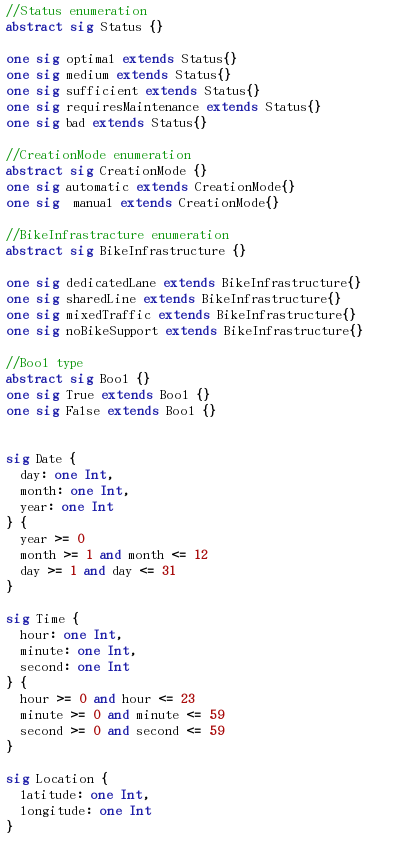
\includegraphics[width=0.55\linewidth]{Images/Alloy/Alloy1.png}
\end{figure}
\begin{figure}[H]
    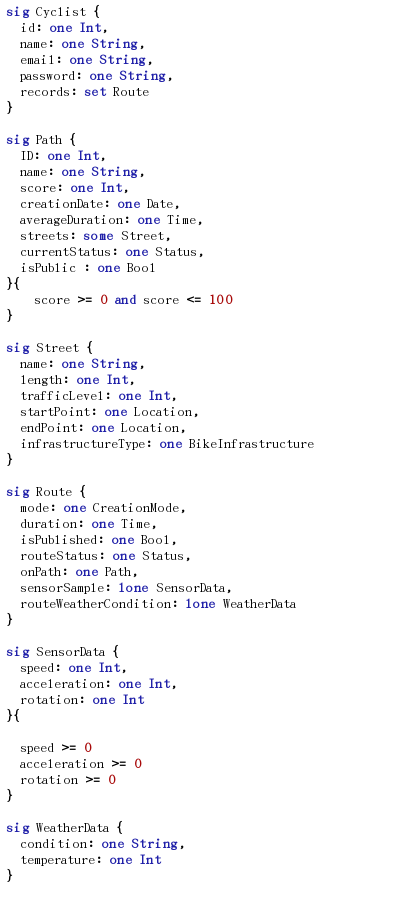
\includegraphics[width=0.65\linewidth]{Images/Alloy/Alloy2.png}
\end{figure}
\newpage
\begin{figure}[H]
    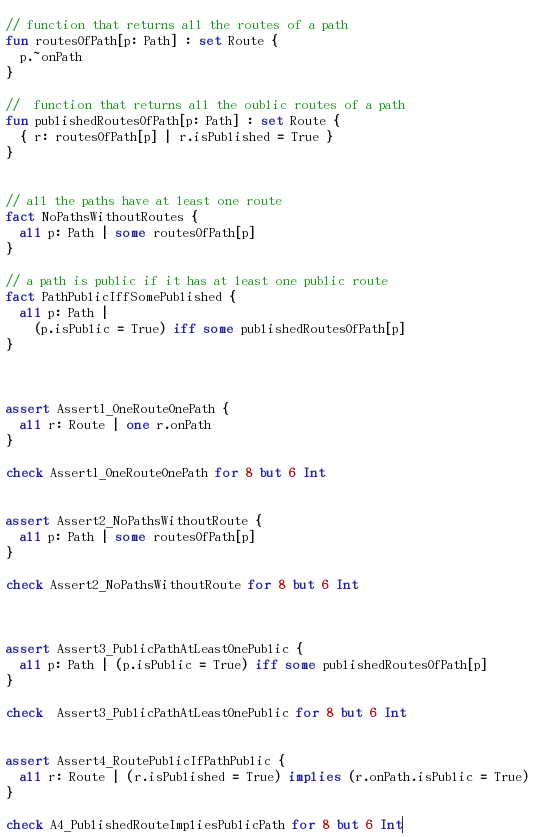
\includegraphics[width=0.75\linewidth]{Images/Alloy/Alloy3.png}
\end{figure} 
\noindent
Finally, we validated the correctness of our model writing several assertions and then checking the correctness of our model (all checks do not find any counterexample). In addition, we run a generic predicate, without any constraint, to confirm that the model is satisfiable and that there exist concrete instances that satisfy all facts and constraints.\\
This step provides evidence that the specification is coherent and that the conceptual model designed for the application can be instantiated consistently.
\newpage
\subsection{Static Analysis With A Simplified Model}
The analysis continues by introducing a simplified version of the model. The goal of this abstraction is not to change the system requirements, but to make  the generated instances easier to read and interpret within Alloy's visualizer. This because the complete model produces a large number of atoms and relations that does not permit a clear visualization of the different behaviors of our model.
\begin{figure}[H]
    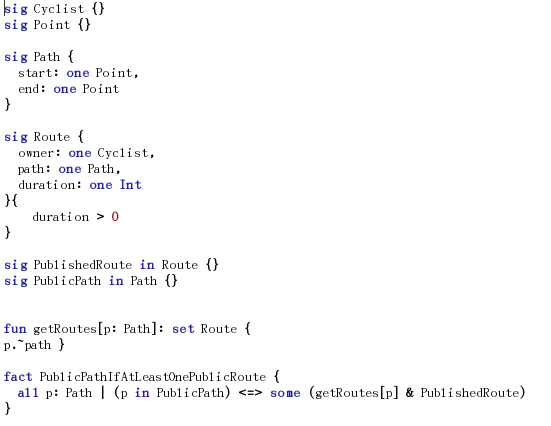
\includegraphics[width=0.65\linewidth]{Images/Alloy/Alloy4.png}
\end{figure}
\noindent The simplified model keeps only the core concept of Cyclist, Route and Path and all details data are removed. Now a path is represented only by start and end points while a Route keeps just the owner, the path and the duration. The publication concept is modeled as subsets: PublishedRoute and PublicPath. 
\begin{figure}[H]
    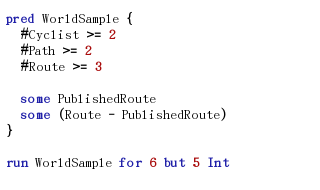
\includegraphics[width=0.37\linewidth]{Images/Alloy/Alloy5.png}
\end{figure}
\begin{figure}[H]
    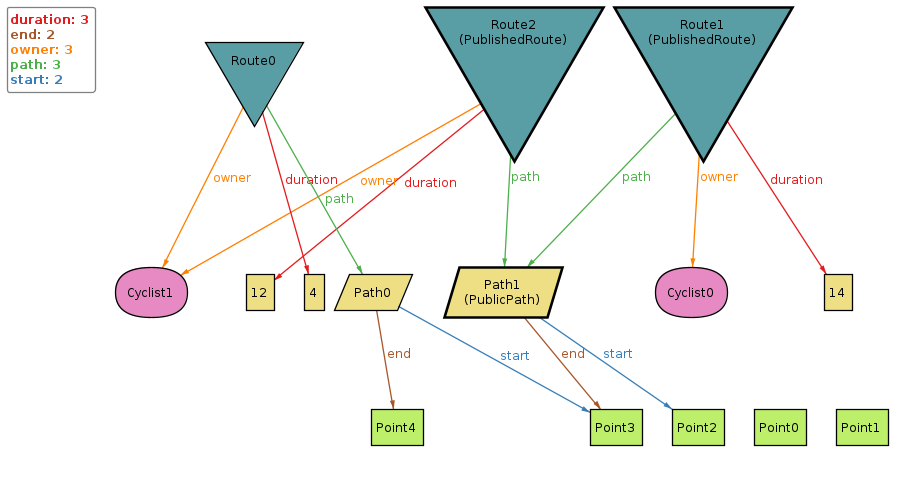
\includegraphics[width=0.6\linewidth]{Images/Alloy/SampleWorld.png}
\end{figure}
\noindent This predicate, WordlSample, shows a generic world with different routes, private and public paths and two cyclists.
\newpage
\begin{figure}[H]
    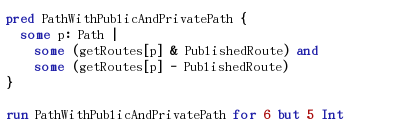
\includegraphics[width=0.5\linewidth]{Images/Alloy/Alloy6.png}
\end{figure}
\begin{figure}[H]
    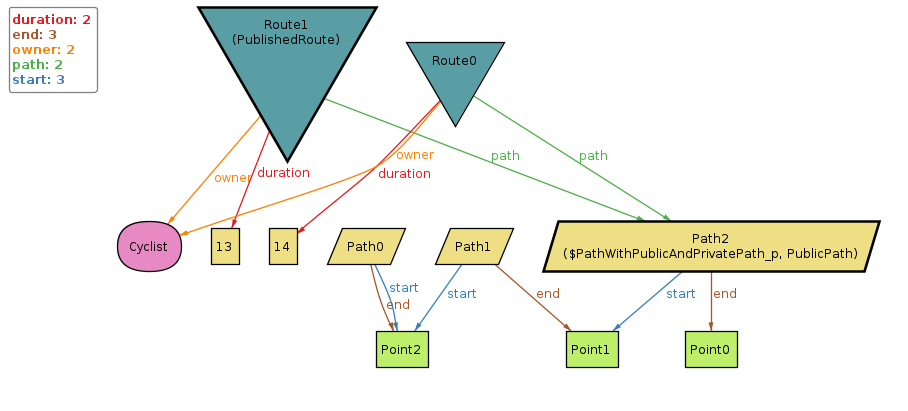
\includegraphics[width=0.5\linewidth]{Images/Alloy/PublichPrivateOnSamePath.png}
\end{figure}
\noindent This instance shows an important property of the system. If a path contains at least one published route, then the path is public even if it also contains private routes. In BPP, only published routes are visible to other users but private routes are still linked to the same path at the data level. This avoids creating a separate “private copy” of the same path. In this way if a cyclist decides to publish a previously private route it will automatically belong to the correct existing public path, preventing duplicates of the same path in the system.
\begin{figure}[H]
    
\includegraphics[width=0.5\linewidth]{RASD - BellomoPenninoSamarani/Images/Alloy/Alloy7.png}
\end{figure}

\begin{figure}[H]
    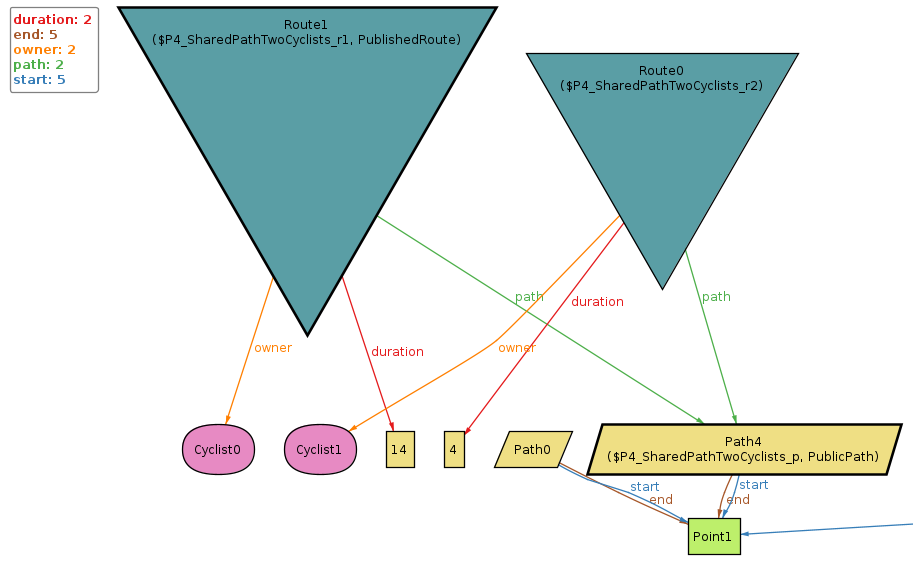
\includegraphics[width=0.5\linewidth]{Images/Alloy/SharedPath.png}
\end{figure}
\noindent This predicate shows the community aspect of BPP where a single path can aggregate multiple routes performed by different Cyclists.
\newpage
\subsection{ Dynamic Analysis }
Dynamic analysis helps to understand how model entities evolve over key operations and is performed on a simplified model, consistent with the approach adopted for static analysis. State changes and system behavior over time were described using the built-in support provided by Alloy 6.
\begin{figure}[H]
    
\includegraphics[width=0.65\linewidth]{RASD - BellomoPenninoSamarani/Images/Alloy/Alloy8.png}
\end{figure}
\newpage
\begin{figure}[H]
    
\includegraphics[width=0.65\linewidth]{RASD - BellomoPenninoSamarani/Images/Alloy/Alloy9.png}
\end{figure}
\noindent The dynamic model represents the system evolution through a mutable relation onPath and a mutable set PublishedRoute. It is forced an initial state, Init. 
The predicates CreateNew, CreateExisting, Publish, Unpublish, Delete model the key operations of the BPP.

\newpage
\begin{figure}[H]
    
\includegraphics[width=0.75\linewidth]{RASD - BellomoPenninoSamarani/Images/Alloy/Alloy10.png}
\end{figure}
\begin{figure}[H]
    
\includegraphics[width=0.55\linewidth]{RASD - BellomoPenninoSamarani/Images/Alloy/d1step0.png}
\end{figure}
\begin{figure}[H]
    
\includegraphics[width=0.55\linewidth]{RASD - BellomoPenninoSamarani/Images/Alloy/d1step1.png}
\end{figure}
\begin{figure}[H]
    
\includegraphics[width=0.55\linewidth]{RASD - BellomoPenninoSamarani/Images/Alloy/d1step2.png}
\end{figure}
\noindent This predicate shows a trace in which a first route is recorded and a new path is created (activated). Additional routes are then added and linked to the same path. The key point is that the system reuses the existing path instead of creating duplicates.

\newpage
\begin{figure}[H]
    
\includegraphics[width=0.55\linewidth]{RASD - BellomoPenninoSamarani/Images/Alloy/Alloy11.png}
\end{figure}
\begin{figure}[H]
    
\includegraphics[width=0.65\linewidth]{RASD - BellomoPenninoSamarani/Images/Alloy/d2step0.png}
\end{figure}
\begin{figure}[H]
    
\includegraphics[width=0.55\linewidth]{RASD - BellomoPenninoSamarani/Images/Alloy/d2step1.png}
\end{figure}
\begin{figure}[H]
    
\includegraphics[width=0.55\linewidth]{RASD - BellomoPenninoSamarani/Images/Alloy/d2step2.png}
\end{figure}
\noindent This predicate shows a route that is initially private and then becomes published. After the publish operation, the route is added to PublishedRoute and its associated path becomes part of PublicPath.

\newpage
\begin{figure}[H]
    
\includegraphics[width=0.65\linewidth]{RASD - BellomoPenninoSamarani/Images/Alloy/Alloy12.png}
\end{figure}
\begin{figure}[H]
    
\includegraphics[width=0.55\linewidth]{RASD - BellomoPenninoSamarani/Images/Alloy/d3step0.png}
\end{figure}
\begin{figure}[H]
    
\includegraphics[width=0.55\linewidth]{RASD - BellomoPenninoSamarani/Images/Alloy/d3step1.png}
\end{figure}
\begin{figure}[H]
    
\includegraphics[width=0.55\linewidth]{RASD - BellomoPenninoSamarani/Images/Alloy/d3step2.png}
\end{figure}
\noindent This is the opposite situation of the previous case. Initially, a route is published, making its path public. When the route is later unpublished and the path has no remaining published routes, the path is no more publish.

\newpage
\begin{figure}[H]
    
\includegraphics[width=0.65\linewidth]{RASD - BellomoPenninoSamarani/Images/Alloy/Alloy13.png}
\end{figure}
\begin{figure}[H]
    
\includegraphics[width=0.55\linewidth]{RASD - BellomoPenninoSamarani/Images/Alloy/d4step0.png}
\end{figure}
\begin{figure}[H]
    
\includegraphics[width=0.55\linewidth]{RASD - BellomoPenninoSamarani/Images/Alloy/d4step1.png}
\end{figure}
\noindent In this case, a path is created with a single route, and then the last route is removed. Since the path no longer contains any routes, it is considered inactive, modeling the cleanup of an empty path.
\subsection{ Conclusions from Alloy Model Analysis}
The alloy analysis provides a clear formal validation of the application model. Through static analysis, the main entities, relationships and global constraints were checked for consistency, demonstrating that valid instances are admitted.\\
Dynamic analysis models the key operations over time showing how routes and paths evolve through creation, publication, and deletion.
These results clarify the intended behavior of the system and offer strong guidance for implementing the application without inconsistencies.